\documentclass[12pt]{report}
\usepackage[a4paper]{geometry}
                		% See geometry.pdf to learn the layout options. There are lots.
\geometry{a4paper}
\usepackage{listings}
\usepackage[cm]{fullpage}
\usepackage{layout}
\usepackage{amsthm}
\usepackage{amssymb,amsmath,amsfonts,latexsym,dsfont}

\usepackage{ upgreek }
\usepackage{xcolor}
\usepackage{titlesec}
\usepackage{mathrsfs}
\usepackage{mathtools}
\usepackage[warn]{mathtext}
\usepackage[T1,T2A]{fontenc}
\usepackage{titlesec, blindtext, color}
\definecolor{gray75}{gray}{0.75}
\newcommand{\hsp}{\hspace{20pt}}
\usepackage[utf8]{inputenc}
\usepackage{fancyhdr}
\usepackage[parfill]{parskip}
\usepackage[english,bulgarian,ukrainian,russian]{babel}
\titleformat{\section}[block]{\color{black}\Large\bfseries\filcenter}{}{1em}{}
\titleformat{\chapter}[hang]{\Huge\bfseries}{\thechapter\hsp\textcolor{gray75}{|}\hsp}{0pt}{\Huge\bfseries}
\setcounter{secnumdepth}{0}
\renewcommand{\le}{\leqslant} 
\renewcommand{\ge}{\geqslant }
\DeclareMathOperator{\sign}{sign}
\DeclareMathOperator*{\argmax}{arg\,max}
\DeclareMathOperator*{\argmin}{arg\,min}
\DeclareMathOperator{\Tr}{Tr}
\DeclareMathOperator{\rg}{rg}
\DeclareMathOperator{\diag}{diag}
\DeclareMathOperator{\cov}{cov}
\DeclareMathOperator{\proj}{proj}

           		% ... or a4paper or a5paper or ... 
%\geometry{landscape}                		% Activate for rotated page geometry
%\usepackage[parfill]{parskip}    		% Activate to begin paragraphs with an empty line rather than an indent
\ifx\pdfoutput\undefined
\usepackage{graphicx}
\else
\usepackage[pdftex]{graphicx}
\lstset{language=C++}
\usepackage{pgffor}
\newcounter{SortListTotal}
\newcommand{\sortitem}[2]{\expandafter\def\csname SortListItem#1\endcsname{#2}\stepcounter{SortListTotal}}
\newcommand{\printsortlist}{\foreach\currentlistitem in{1,2,...,\value{SortListTotal}}{\item[\currentlistitem]\csname SortListItem\currentlistitem\endcsname}\setcounter{SortListTotal}{0}}
\newcommand\setItemnumber[1]{\setcounter{enumi}{\numexpr#1-1\relax}}

\title{Метод Монте-Карло для моделирования ферромагнетиков}
\author{Никита Балаганский, Артем Ямалутдинов}
\date{\today}

\usepackage{natbib}
\usepackage{graphicx}
\renewenvironment{proof}{{\bfseries Доказательство:}}{$\square$\\\\}
\newenvironment{solution}{{\bfseries Решение:}}{$\square$\\\\}
\newtheorem{theorem}{Теорема}
\newtheorem{lemma}{Лемма}
\newtheorem{proposition}{Утверждение}
\newtheorem{corollary}{Следствие}
\theoremstyle{definition}
\newtheorem{definition}{Определение}
\newtheorem{notation}{Обозначение}
\newtheorem{example}{Пример}
\newtheorem{problem}{Задача}
\newtheorem{sense}{Смысл}
\newtheorem{remark}{Замечание}
\newcommand{\vect}[1]{\boldsymbol{#1}}

\begin{document}
\maketitle
\fancyhead[C]{field}
\fancyfoot[C]{МФТИ}%
\thispagestyle{fancy}
\newpage
\chapter{Введение}
\section{1.1. Ферромагнетизм}
\emph{Ферромагнетиками} называются твердые тела, которые могут обладать \emph{спонтанной намагниченностью}, т. е. намагничены уже в отсутствие магнитного поля.
Типичными представителями ферромагнетиков являются железо, кобальт, никель и многие их сплавы. Ферромагнетизмом обладают многие редкоземельные элементы при пониженной температуре.

Атомы железа, никеля, кобальта в кристаллах располагаются таким образом, что собственные магнитные поля неспаренных электронов оказываются направленными параллельно друг другу и внутри кристалла образуются микроскопические намагниченные области – \emph{домены}.
В разных доменах ориентация магнитного поля различна, их суммарное магнитное поле равно нулю. 
При помещении во внешнее магнитное поле внутренние магнитные поля доменов ориентируются по направлению внешнего поля, ферромагнетик намагничивается.

Упорядоченное расположение магнитных полей электронов в доменах ферромагнетиков при достаточно высокой температуре разрушается беспорядочными тепловыми колебаниями атомов в узлах кристаллической решётки.
Температура , выше которой ферромагнитное вещество теряет свои ферромагнитные свойства, называется \emph{температурой Кюри} или \emph{точкой Кюри}.

\section{1.2. Модель Изинга}
Модель Изинга --- одна из основных моделей, описывающая поведение магнитных моментов 
в атомах ферромагнетика выше точки Кюри $T_C$. В данной модели каждой вершине кристаллической решетки ставится в соответствие число $+1$ или $-1$, 
отвечаюее за противоположные направления магнитного момента. Это число называется \emph{спином}. Тогда в отсутствие внешнего магнитного поля гамильтониан получившейся системы можно записать в виде
\begin{equation}\label{eq:energy}
    \mathcal{H} = -J\sum_{\langle i, j \rangle}s_is_j,
\end{equation}
где $\langle i, j \rangle$ означает суммирование по соседним элементам,  $J > 0$ --- энергия взаимодействия соседних спинов (считаем ее одинаковой для всех пар),
$s_i, s_j$ --- спины.

При температуре $T_C$ система испытывает \emph{фазовый переход второго рода}.

Покажем, что если кристаллическая решетка одномерная, то фазовый переход в ней невозможен, т.е при любых температурах
упорядоченное состояние энергетически невыгодно.
Для этого запишем \emph{свободную энергию системы}
\begin{equation}
    F = E - TS.
\end{equation}
Здесь  $E$ --- энергия, $S$ --- энтропия системы. Упорядоченное состояние будет устойчиво тогда и только тогда, когда
при переходе в него $\Delta F > 0$.

Изменим спины таким образом, чтобы в системе появился упорядоченный домен. Тогда энергия увеличится на величину $4J$, а изменение энтропии
$\Delta S = k_B \ln N$, где $N$ --- число атомов в решетке. Тогда изменение свободной энергии
\begin{equation}
    \Delta F = 4J - k_B T \ln N < 0 \text{ при }N \to \infty,
\end{equation}
то есть для системы неупорядоченное состояние более выгодно.

Теперь рассмотрим двумерный случай. При введении домена в кристаллическую решетку изменение энергии системы пропорционально периметру домена и может быть записано как
$\Delta E = 4J \cdot \varepsilon N^2, \quad 0 < \varepsilon < 1$. Возможное число доменов можно оценить как  $3^{\varepsilon N^2}$. Тогда изменение энергии
\begin{equation}
    \Delta F = 4J \cdot \varepsilon N^2 - k_B T \ln (N^2 3^{\varepsilon N^2}).
\end{equation}
Отсюда можно получить оценку на точку Кюри $T_C$:
\begin{equation}
    T_C \sim \dfrac{J}{k_B}.
\end{equation}
Более аккуратный подсчет дает теоретическую оценку точки Кюри $T_C = \frac{2J}{k_B\ln(1 + \sqrt{2})} \approx 2.27\frac{J}{k_B}.$
\chapter{Метод Монте-Карло}
\section{2.1. Описание метода}
Для системы из $N$ спинов число возможных состояний равно $2^N$, поэтому
для моделирования систем с достаточно большим $N$ необходимо использовать статистические методы.

В методе Монте-Карло система рассматривается в состоянии термодинамического равновесия при
определенной температуре $T$. В ходе обмена энергией с окружающей средой, энергия будет
флуктуировать около равновесного состояния, а средняя энергия одной частицы пропорциональна $T$.
Тогда для подсчета термодинамических характеристик системы можно будет посчитать ее характеристики для реализованных состояний,
а далее усреднить получившиеся значения.
\section{2.2. Алгоритм Метрополиса}
Описание алгоритма, используемого для моделирования кристаллической решетки ферромагнетика:
\emph{Алгоритм 1}
\begin{enumerate}
    \item Случайным образом выбирается начальная конфигурация из $N$ спинов $\alpha_0$;
    \item На $k$-ом шаге меняем направление одного случайно выбранного спина и считаем изменение энергии $dE$;
    \item Если $dE < 0$, то новое состояение $\alpha_k$ принимается с вероятностью $1$. 
    Если $dE > 0$, то принимаем новое состояние с вероятностью $P = e^{\frac{-dE}{k_B T}}$;
    \item Повторяем шаги $2-4$, принимая $\alpha_k$ в качестве нового исходного состояния.
    \label{alg_metropolis}
\end{enumerate}
\newpage
\section{2.3. Марковские цепи}
Модель Изинга можно рассматривать как марковскую цепь, так как непосредственная вероятность $P_{\beta}(a \rightarrow b)$ перехода в следующее состояние
$b$ зависит только от текущего состояния $a$. Алгоритм Метрополиса на самом деле является версией моделирования Марковской цепи Монте-Карло, и поскольку мы используем динамику с одним
спином в алгоритме Метрополиса, каждое состояние можно рассматривать как точку перехода ровно на $N$ других состояний, где каждый переход соответствует изменению одного спинового момента на противоположное значение.


\begin{figure}[htbp]
    \centering
    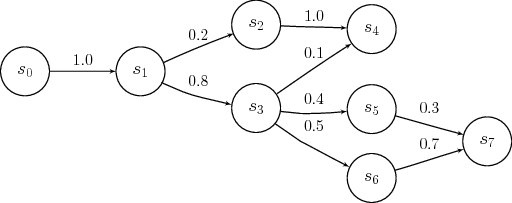
\includegraphics[scale=0.5]{img/markov_chain.png}
\end{figure}

Для того, чтобы алгоритм можно было использовать необходимо найти такое распределение $\pi$, что:
\begin{equation}\label{eq:equlibrium}
    \pi(a)p(a \rightarrow b) = \pi(b)p(b \rightarrow a)
\end{equation}

Давайте докажем, что при выборе $\pi(a) = \frac{1}{Z} \exp{\left(-\frac{E_a}{k_B T}\right)}$ условие $(2.1)$ выполнено.
Итак, пусть
$$
\left\{\begin{array}{l}{p_{a \rightarrow b}=\exp \left(-\frac{E_{b}-E_{a}}{k_B T}\right)} \\ {p_{b \rightarrow a}=1}\end{array}\right.
$$
Тогда $\pi(a) = \pi(b) \cdot \exp \left(-\frac{E_{b}-E_{a}}{k_B T}\right)$.
Подставивив $\pi(a) = \frac{1}{Z} \exp{\left(-\frac{E_a}{k_B T}\right)}$ и $\pi(b) = \frac{1}{Z} \exp{\left(-\frac{E_b}{k_B T}\right)}$
получим верное тождество. В случае $p(a \rightarrow b) = 0$, мгновенно получим $p(b \rightarrow a) = 0$.
\newline
Также необходимо учитывать что для достижения некоррелированности от предыдущего состояния приходится совершать внушительное числло итераций
алгоритма (нужно достаточно глубоко зайти в граф марковской цепи).

\section{2.4. Подсчет термодинамических характеристик системы}
Алгоритм Метрополиса позволяет не только моделировать возможные ориентации магнитных моментов атомов ферромагнетика, но и оценить термодинамические параметры системы.
Для того, чтобы оценить энергию, которой обладает ферромагнетик, необходимо для каждой реализации алгоритма Метрополиса 
посчитать гамильтониан системы по формуле $(1.1)$ и усреднить получившиеся значения. Другими словами,
\begin{equation}
    E = \langle \mathcal{H} \rangle.
\end{equation}
Намагниченность материала $I$ можно оценить похожим образом: достаточно посчитать сумму магнитных моментов $s_i$ для каждой реализации и усреднить их:
 \begin{equation}
    I = \langle \sum_{i = 1}^N s_i \rangle.
\end{equation}
Очевидно, что при $T > T_C \;\; I = 0$.

\noindent Для магнитной восприимчивости $\chi$ получим следующую формулу (равенство следует из теорем статистической термодинамики):
\begin{equation}
    \chi = \frac{1}{N}\frac{\partial I}{\partial h} = \frac{1}{Nk_BT}(\langle M^2 \rangle - \langle M \rangle^2).
\end{equation}
Формулу $(2.4)$ можно переписать в виде
\begin{equation}
    \chi = \frac{1}{k_BT}\sum_{i, j = 1}^N \langle s_is_j \rangle - \langle s_i \rangle \langle s_j \rangle.
\end{equation}
Наконец, для теплоемкости $C$ имеем формулу
\begin{equation}
    C = \frac{\partial E}{\partial T} = -\frac{1}{k_BT^2}\frac{\partial E}{\partial \beta} = \frac{\sigma^2_E}{k_BT^2},
\end{equation}
где $\beta = \frac{1}{k_BT}, \, \sigma_E^2 =  \langle E^2 \rangle - \langle  E \rangle^2$. Можно показать, что $C \sim \ln |T - T_C| \text{ при } T \to T_C$.


\chapter{Appendix}

\begin{figure}[hbtp]
    \centering
    
\includegraphics[scale=0.3]{img/low_t.png}
    \caption{Структура ферромагнетика при температуре ниже точки Кюри}
\end{figure}
\begin{figure}[hbtp]
    \centering
    
\includegraphics[scale=0.3]{img/high_t.png}
    \caption{Структура ферромагнетика при температуре выше точки Кюри}
\end{figure}

\begin{figure}[hbtp]
    \centering
    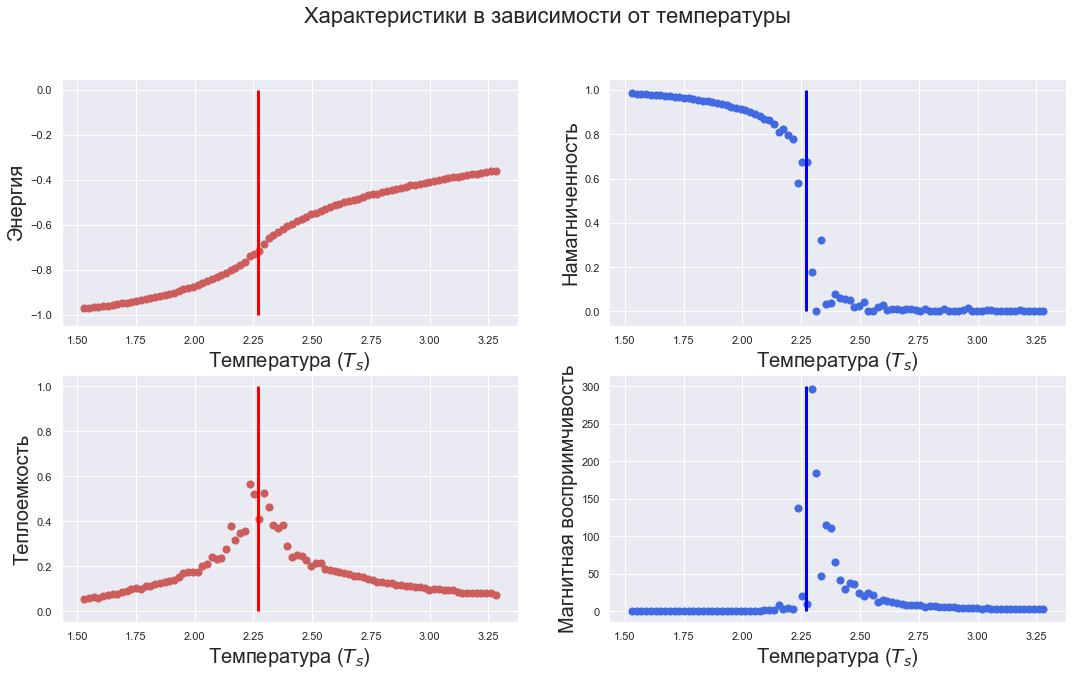
\includegraphics[scale=0.4]{img/temperature.png}
    \caption{Зависимости от температуры. Черта соответствует точке Кюри}
\end{figure}

\begin{figure}[hbtp]
    \centering
    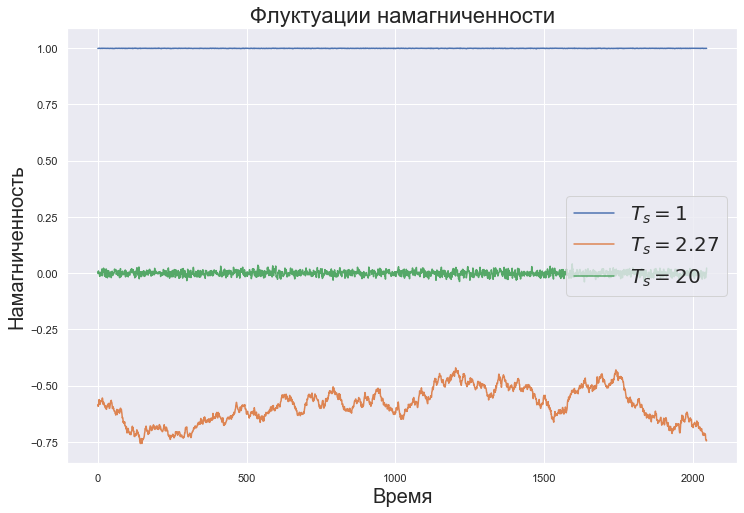
\includegraphics[scale=0.4]{img/fluctuations.png}
    \caption{Флуктуации намагниченности}
\end{figure}

\end{document}
